\clearpage
\VerdierPhysicalPageAnchor{0095}%
\begingroup
\setlength{\abovedisplayskip}{4pt plus 2pt minus 2pt}%
\setlength{\belowdisplayskip}{4pt plus 2pt minus 2pt}%
\VerdierSemanticAnchor{ch1-3-3}
\subsection{Propriétés des triangles distingués}

\VerdierSemanticAnchor{ch1-3-3-1}
\noindent\textbf{Définition 3.3.1.}\quad
\VerdierSemanticAnchor{ch1-3-3-1-distinguished-triangle}
Un triangle
$X\xrightarrow{u}Y\xrightarrow{v}Z\xrightarrow{w}X[1]$ de $K(C)$ sera dit
\emph{distingué} s'il existe un objet
$X'\xrightarrow{\dot f'}Y'$ de $\operatorname{Tr}_1(C)$ et un isomorphisme
de triangles ((3.2.1.3) et (3.2.2.7)) :

\VerdierSemanticAnchor{ch1-3-3-1-isomorphism-diagram}
\begin{center}
  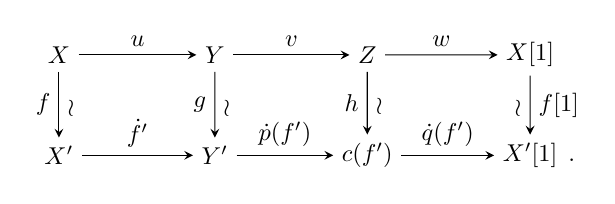
\begin{tikzpicture}[>=stealth,scale=0.88,every node/.style={transform shape}]
    \node (X)   at (0,1.45) {$X$};
    \node (Y)   at (2.25,1.45) {$Y$};
    \node (Z)   at (4.45,1.45) {$Z$};
    \node (Xs)  at (6.80,1.45) {$X[1]$};
    \node (Xp)  at (0,0) {$X'$};
    \node (Yp)  at (2.25,0) {$Y'$};
    \node (Cf)  at (4.45,0) {$c(f')$};
    \node (Xps) at (6.80,0) {$X'[1]$};
    \node[anchor=base west,inner sep=0pt,xshift=.08em] at (Xps.base east) {$.$};
    \draw[->] (X) -- node[above] {$u$} (Y);
    \draw[->] (Y) -- node[above] {$v$} (Z);
    \draw[->] (Z) -- node[above] {$w$} (Xs);
    \draw[->] (Xp) -- node[above] {$\dot f'$} (Yp);
    \draw[->] (Yp) -- node[above] {$\dot p(f')$} (Cf);
    \draw[->] (Cf) -- node[above] {$\dot q(f')$} (Xps);
    \draw[->] (X) -- node[left] {$f$} node[right,pos=.55] {$\wr$} (Xp);
    \draw[->] (Y) -- node[left] {$g$} node[right,pos=.55] {$\wr$} (Yp);
    \draw[->] (Z) -- node[left] {$h$} node[right,pos=.55] {$\wr$} (Cf);
    \draw[->] (Xs) -- node[right] {$f[1]$} node[left,pos=.55] {$\wr$} (Xps);
  \end{tikzpicture}
\end{center}

\VerdierSemanticAnchor{ch1-3-3-2}
\noindent\textbf{Proposition 3.3.2. (TRI)}\quad
\VerdierSemanticAnchor{ch1-3-3-2-isomorphism-invariance}
\textit{Tout triangle de $K(C)$ isomorphe à un triangle distingué est un
triangle distingué.}
\VerdierSemanticAnchor{ch1-3-3-2-identity-triangle}
\textit{Pour tout objet $X$ de $K(C)$, le triangle
$X\xrightarrow{\operatorname{id}_X}X\longrightarrow0\longrightarrow X[1]$
est distingué.}
\VerdierSemanticAnchor{ch1-3-3-2-completion}
\textit{Tout morphisme $u\colon X\to Y$ de $K(C)$ est contenu dans un
triangle distingué
$X\xrightarrow{u}Y\xrightarrow{v}Z\xrightarrow{w}X[1]$.}

\VerdierSemanticAnchor{ch1-3-3-2-proof-first}
La première assertion est triviale. Pour démontrer la deuxième assertion,
il suffit de montrer que le diagramme :

\VerdierSemanticAnchor{ch1-3-3-2-identity-comparison}
\begin{center}
  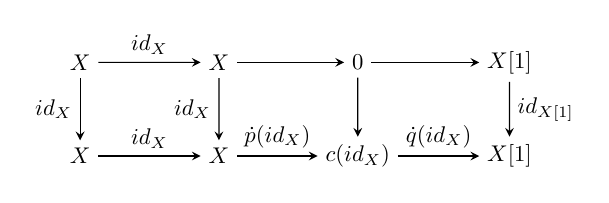
\begin{tikzpicture}[>=stealth,scale=0.82,every node/.style={transform shape}]
    \node (X1) at (0,1.45) {$X$};
    \node (X2) at (2.15,1.45) {$X$};
    \node (Z1) at (4.30,1.45) {$0$};
    \node (Xs1) at (6.65,1.45) {$X[1]$};
    \node (X3) at (0,0) {$X$};
    \node (X4) at (2.15,0) {$X$};
    \node (Cid) at (4.30,0) {$c(\operatorname{id}_X)$};
    \node (Xs2) at (6.65,0) {$X[1]$};
    \draw[->] (X1) -- node[above] {$\operatorname{id}_X$} (X2);
    \draw[->] (X2) -- (Z1);
    \draw[->] (Z1) -- (Xs1);
    \draw[->] (X3) -- node[above] {$\operatorname{id}_X$} (X4);
    \draw[->] (X4) -- node[above] {$\dot p(\operatorname{id}_X)$} (Cid);
    \draw[->] (Cid) -- node[above] {$\dot q(\operatorname{id}_X)$} (Xs2);
    \draw[->] (X1) -- node[left] {$\operatorname{id}_X$} (X3);
    \draw[->] (X2) -- node[left] {$\operatorname{id}_X$} (X4);
    \draw[->] (Z1) -- (Cid);
    \draw[->] (Xs1) -- node[right] {$\operatorname{id}_{X[1]}$} (Xs2);
  \end{tikzpicture}
\end{center}

\VerdierSemanticAnchor{ch1-3-3-2-identity-cone-null}
est un isomorphisme de triangles de $K(C)$. Il suffit donc de montrer que
$c(\operatorname{id}_X)$ est homotope à zéro. Or il résulte immédiatement
de la définition des homotopies dans $\operatorname{tr}_1(C)$ (3.1.4) que
tout morphisme de $\operatorname{tr}_1(C)$ du type :

\VerdierSemanticAnchor{ch1-3-3-2-tr1-null-diagram}
\begin{center}
  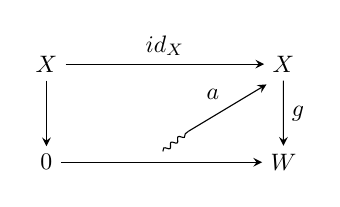
\begin{tikzpicture}[>=stealth,scale=0.86,every node/.style={transform shape}]
    \node (X1) at (0,1.45) {$X$};
    \node (X2) at (3.50,1.45) {$X$};
    \node (Z)  at (0,0) {$0$};
    \node (W)  at (3.50,0) {$W$};
    \draw[->] (X1) -- node[above] {$\operatorname{id}_X$} (X2);
    \draw[->] (X1) -- (Z);
    \draw[->] (X2) -- node[right] {$g$} (W);
    \draw[->] (Z) -- (W);
    \draw[decorate,decoration={snake,amplitude=0.8pt,segment length=3.3pt}]
      (1.72,0.16) -- (2.10,0.46);
    \draw[->] (2.10,0.46) -- node[above left] {$a$} (3.25,1.15);
  \end{tikzpicture}
\end{center}

\VerdierSemanticAnchor{ch1-3-3-2-tr1-null-conclusion}
est homotope à zéro.
\VerdierSemanticAnchor{ch1-3-3-2-adjunction}
Les propriétés d'adjonction du foncteur cône (3.1.6) montrent alors que
$c(\operatorname{id}_X)$ est homotope à zéro.
\VerdierSemanticAnchor{ch1-3-3-2-open-morphism}
Soit $f\colon X\to Y$ un morphisme
\endgroup

